% Created 2021-04-28 mer. 10:16
% Intended LaTeX compiler: pdflatex
\documentclass[presentation]{beamer}
\usepackage[orientation=portrait,size=a0,scale=1.4,debug]{beamerposter}
\usepackage[overlay]{textpos}
\usepackage[utf8]{inputenc}
\usepackage[T1]{fontenc}
\usepackage{graphicx}
\usepackage{alphalph}
\def\theequation{\AlphAlph{\value{equation}}}

\setbeamertemplate{caption}{\raggedright\insertcaption\par}

\newtheorem{assumption}{Assumption}%[numberby]
\newtheorem{remark}{Remark}%[numberby]
\usepackage[ruled,noend,algo2e]{algorithm2e}
\usepackage{fontawesome}
\usepackage{pgfplots}
\usepackage{grffile}
\usepackage{longtable}
\usepackage{wrapfig}
\usepackage{rotating}
\usepackage[normalem]{ulem}
\usepackage{amsmath}
\usepackage{textcomp}
\usepackage{amssymb}
\usepackage{booktabs}
\usepackage{capt-of}
\usepackage{hyperref}
\usepackage{tikz}
\usepackage{circuitikz}
\usetikzlibrary{arrows.meta,calc}
\usetikzlibrary{calc,shapes,positioning,shapes.misc}

\newcommand<>{\script}[1]{\note{\onslide#2{#1}}}


\newif\ifdebug%
\newcommand{\draft}{\debugtrue}
\newcommand{\final}{\debugfalse}
\newcommand{\todo}[2][FORGOT TO DO SOMETHING]{\ifdebug%
  {%
    \color{red}
    #2}\else \PackageError{}{#1}{#2}#2\fi}%
\newcommand\doing[2][FORGOT TO DO SOMETHING]{\ifdebug%
  {%
    \color{blue}
    #2}\else \PackageError{}{#1}{#2}#2\fi}%
\newcommand\warning[1]{\ifdebug%
  {%
    \color{red}
    #1}\fi}

\draft% show todos in red
% \final% give error if there is todos

% \usepackage[french]{babel}
\usepackage[english]{babel}
\usepackage{amsmath}
\usepackage{graphicx}
\usepackage[utf8]{inputenc}
\usepackage{pgfpages}
\usepackage{multicol}
\usepackage{totcount}
\regtotcounter{section}

\usepackage{amsmath}
\usepackage{mathtools}
\usepackage{amssymb}
\usepackage{picture}
\usepackage{bbding}
\usepackage{bbold}
\usepackage{sansmathaccent}
\pdfmapfile{+Sensationsmache.map}
\usepackage{stmaryrd}
\usepackage{tikz}

% \newcommand\warning[1]{\ifdebug {\color{red}#1}\fi}

\usepackage{hyperref}
\usepackage{natbib}
\usepackage[thicklines]{cancel}
\renewcommand{\CancelColor}{\color{red}}
\usepackage{ulem}

\usetheme{default}
\author{{\bfseries Rafael Accácio Nogueira}, Romain Bourdais, Simon Leglaive, Hervé Guéguen}


\date{\today}
\title{Expectation-Maximization Based Defense Mechanism  \\for Distributed Model Predictive Control}
\institute{IETR-CentraleSupélec, Rennes, France}
\subtitle{The Subtitle}
\usepackage{beamerthemeIETRposter}


\email{rafael-accacio.nogueira\\@centralesupelec.fr}

\usepackage{appendixnumberbeamer}
\usepackage{ amssymb }

\definecolor{mpc_agent}{RGB}{39,154,216}
\definecolor{mpc_agent_foreground}{RGB}{39,154,216}
\colorlet{mpc_agent_foreground}{black}
\definecolor{mpc_agent}{RGB}{243, 146, 0} % logo necsys
% \definecolor{mpc_agent}{RGB}{169, 195, 124} % verde Eve
% \definecolor{mpc_agent}{RGB}{128, 149, 117} %
% \definecolor{mpc_agent}{RGB}{46, 182, 255} % original with more V in HSV
\definecolor{mpc_green}{RGB}{98, 160, 98}
\definecolor{mpc_coordinator}{RGB}{235, 235, 235}
\definecolor{mpc_orange}{RGB}{247, 153, 68}
\definecolor{mpc_yellow}{RGB}{245, 235, 103}
% \usepackage{graphicx}      % include this line if your document contains figures
\usepackage{grffile}       % filenames
\usepackage{booktabs}       % filenames
\usepackage{xparse}
% \usepackage{hyperref}
\usepackage{tikz}
\usetikzlibrary {graphs}

\usepackage{tikzscale}
\usepackage{bm}
\usepackage{ifthen}
\usepackage[ruled,noend,algo2e]{algorithm2e}
\SetKwRepeat{Do}{do}{while}

\usepackage[justification=centering]{caption}
\usepackage{subcaption}
% \usepackage{pdfcomment}


% \newcommand{\symbl}[3]{\newglossaryentry{#1}{name ={#2},	description ={#3}}
%   \expandafter\newcommand\csname #1\endcsname{\gls{#1}}
% }




\usepackage{color}
\newcommand{\no}[1]{}

\def\maybeonecolumn{}

\makeatletter
\def\comments{
  \usepackage{geometry}
  \newgeometry{
    textwidth=8cm,
    hoffset=-1.5in,
    bottom=0.41in,
    vscale=.5,
    % height=.2\textheight,
    top=0.41in,
    footskip=1cm,
  }
\@TwoColumnfalse
\@twocolumnfalse
}
\makeatother

% \usepackage{stfloats}

% \usepackage[showframe]{geometry}
% \usepackage{geometry}
% \geometry{
%   top=19.1mm,
%   bottom=36.7mm,
%   left=19.1mm,
%   right=13.1mm,
% }



\newif\ifdebug%
\newcommand{\draft}{\debugtrue}
\newcommand{\final}{\debugfalse}
\newcommand{\todo}[2][FORGOT TO DO SOMETHING]{\ifdebug%
  {
    \color{red}
    #2}\else \PackageError{}{#1}{#2}#2\fi}%
\newcommand\doing[2][FORGOT TO DO SOMETHING]{\ifdebug%
  {
    \color{blue}
    #2}\else \PackageError{}{#1}{#2}#2\fi}%
\newcommand\warning[1]{\ifdebug%
  {
    \color{red}
    #1}\fi}

\makeatletter
\@ifpackageloaded{pdfcomment}
{
  \newcommand\pdfnote[1]{
    \ifdebug%
    {\pdfcomment[color=orange,opacity=0.4,subject=note]{#1}
    }\fi
  }
  \newcommand{\question}[1]{
    \ifdebug%
    {\pdfcomment[color=red,opacity=0.4,subject=Should I?]{#1}
    }\fi}
}
{
  \newcommand\pdfnote[1]{
    \ifdebug%
    {\tikz[opacity=.7]{\node[text width=2cm,align={center},color=black,fill=red,draw] {#1} }
    }\fi
  }
  \newcommand{\question}[1]{
    \ifdebug%
    {\tikz[opacity=.7]{\node[text width=2cm,align={center},rotate=2,color=black,fill=orange,draw] {#1} }
    }\fi
  }
}
\makeatother
% \newcommand\pdfnote[1]{}


%===============================================================================
\newtheorem{theorem}{theorem}[section]
\newtheorem{problem}[thm]{Problem}%[numberby]
\newtheorem{example}{Example}%[numberby]
\newtheorem{remark}{Remark}%[numberby]
\newtheorem{assumption}{Assumption}%[numberby]

\graphicspath{{../img/}}

% \makeatletter
% \hypersetup{
%   bookmarks=true,         % show bookmarks bar?
%   unicode=false,          % non-Latin characters in Acrobat’s bookmarks
%   pdftoolbar=true,        % show Acrobat’s toolbar?
%   pdfmenubar=true,        % show Acrobat’s menu?
%   pdffitwindow=false,     % window fit to page when opened
%   pdfstartview={FitH},    % fits the width of the page to the window
%   pdftitle={\@title},    % title
%   pdfauthor={\@author},     % author
%   pdfsubject={},   % subject of the document
%   pdfcreator={Rafael Accácio},   % creator of the document
%   % pdfproducer={Producer}, % producer of the document
%   pdfkeywords={keyword1, key2, key3}, % list of keywords
%   pdfnewwindow=true,                  % links in new PDF window
%   colorlinks=true,            % false: boxed links; true: colored links
%   % colorlinks=false,            % false: boxed links; true: colored links
%   linkcolor=black, % color of internal links (change box color with linkbordercolor)
%   citecolor=black,          % color of links to bibliography
%   filecolor=black,          % color of file links
%   urlcolor=black            % color of external links
% }
% \makeatother



\newcommand{\eq}[2]{\mbox{$#1=#2$}}
\newcommand{\N}{\mathbb{N}}
\newcommand{\Z}{\mathbb{Z}}
\newcommand{\Q}{\mathbb{Q}}
\newcommand{\R}{\mathbb{R}}
\newcommand{\C}{\mathbb{C}}
\newcommand{\Np}{N_{\text{p}}}
\newcommand{\T}{^{\mathrm{T}}}
\newcommand{\1}{\mathbf{1}}
\newcommand{\0}{\mathbf{0}}
\newcommand{\abs}[1]{\left\lvert#1\right\rvert}
\newcommand{\norm}[1]{\left\lVert#1\right\rVert}
\newcommand{\Varepsilon}{\mathcal{E}}
\newcommand{\diff}{\mathop{}\mathopen{}\mathrm{d}}
\newcommand{\set}[1]{\mathcal{#1}}
\newcommand{\p}{^{(p)}}
\newcommand{\pplusone}{^{(p+1)}}
\renewcommand{\vec}[1]{\boldsymbol{#1}}
\newcommand{\random}[1]{\underline{#1}}
\newcommand{\randomvec}[1]{{\underline{\vec{#1}}}}
\newcommand{\probability}[1]{\mathbb{P}(#1)}
\newcommand{\expectation}[2][]{\mathbb{E}_{#1}\left[#2\right]}
\newcommand{\indicator}[1]{\mathbb{1}_{\{#1\}}}

\newcommand{\setbuild}[2]{\{#1\mid#2\}}
\newcommand{\seq}[2][n]{\lbrace #2_{0},\ldots,\,#2_{#1} \rbrace}
\newcommand{\hadamard}[2]{#1\odot #2}
\newcommand{\kron}[2]{#1\otimes#2}
\newcommand{\vectorize}[1]{\mathrm{vec} (#1)}
\newcommand{\symmetric}{\mathbb{S}}
\newcommand{\semidefpos}{\mathbb{S}_{+}}
\newcommand{\defpos}{\mathbb{S}_{++}}
\newcommand{\elem}[2][1]{{#2}_{(#1)}}
\newcommand{\pseudoinv}[1]{{#1}^{\dagger}}
% \renewcommand{\implies}{\Rightarrow}
% \renewcommand{\iff}{\Leftrightarrow}



\usepackage{amsmath}
\usepackage{mathtools}
\usepackage{amssymb}
\DeclareMathOperator{\fix}{fix}
\DeclareMathOperator{\diag}{diag}
\DeclareMathOperator{\Proj}{Proj}
\DeclareMathOperator{\dom}{dom}
\DeclareMathOperator{\argmax}{arg\ max}
% \DeclareMathOperator{\card}{\#}
\newcommand{\card}[1]{\#(#1)}
% \DeclareMathOperator{\vector}{vec}
%

% Theorem
% \newtheorem{thm}{Theorem}[section]
% \newtheorem{lem}[thm]{Lemma}

\newcommand{\nsubsystems}{M}
\newcommand{\umax}{\vec{u}_{\mathrm{\max}}}
\newcommand{\predhorz}{N_{p}}

\NewDocumentCommand \mpcvec { s m o o o } {%
  \IfBooleanTF{#1}{
    \def\optim{^\star}
  }{
    \def\optim{}
  }
  \IfValueTF{#5}{
    \vec{#2}_{#3}\optim{}[#4|#5]
  }{
    \IfValueTF{#4}{
      \vec{#2}_{#3}\optim{}[#4]
    }
    {
    \IfValueTF{#3}{
      \vec{#2}_i\optim{}[#3]
    }
    {
      \vec{#2}_i\optim{}[k]
    }
    }
  }
}


\NewDocumentCommand \mpcval { s m o o o } {%
  \IfBooleanTF{#1}{
    \def\optim{^\star}
  }{
    \def\optim{}
  }
  \IfValueTF{#5}{
    {#2}_{#3}\optim{}[#4|#5]
  }{
    \IfValueTF{#4}{
      {#2}_{#3}\optim{}[#4]
    }
    {
    \IfValueTF{#3}{
      {#2}_i\optim{}[#3]
    }
    {
      {#2}_i\optim{}[k]
    }
    }
  }
}






\newcommand{\uikk}{\mpcvec{u}[i][k][k]}
\newcommand{\optuikk}{\mpcvec*{u}[i][k][k]}

\newcommand{\globobj}{\mpcval{J}[][k]}
\newcommand{\optglobobj}{\mpcval*{J}[][k]}

\newcommand{\obji}{\mpcval{J}[i][k]}
\newcommand{\optobji}{\mpcval*{J}[i][k]}

\newcommand{\xik}{\mpcvec{x}}
\newcommand{\fik}{\mpcvec{f}}
\newcommand{\uik}{\mpcvec{u}}
\newcommand{\uiseq}{\mpcvec{u}[i][k:k+\predhorz-1][k]}
\newcommand{\optuiseq}{\mpcvec*{u}[i][k:k+\predhorz-1][k]}

\newcommand{\useq}{\mpcvec{u}[ ][k:k+\predhorz-1][k]}
\newcommand{\optuseq}{\mpcvec*{u}[ ][k:k+\predhorz-1][k]}
\newcommand{\Uik}{\mpcvec{U}}
\newcommand{\optUik}{\mpcvec*{U}}
\newcommand{\optuncUik}{\mpcvec*{\mathring{U}}}

\newcommand{\vik}{\mpcvec{v}}
\newcommand{\wik}{\mpcvec{w}}
\newcommand{\wiseq}{\mpcvec{w}[i][k:k+\predhorz-1][k]}
\newcommand{\Wik}{\mpcvec{W}}

\newcommand{\qik}{\mpcvec{q}}
\newcommand{\qiseq}{\mpcvec{q}[i][k:k+\predhorz-1][k]}
\newcommand{\thetaik}{\mpcvec{\theta}}
\newcommand{\optthetaiseq}{\mpcvec*{\theta}[i][k:k+\predhorz-1][k]}
\newcommand{\thetaseq}{\mpcvec{\theta}[][k:k+\predhorz-1][k]}
\newcommand{\optthetaseq}{\mpcvec*{\theta}[][k:k+\predhorz-1][k]}
\newcommand{\thetai}{\vec{\theta}_i}
\newcommand{\optthetai}{\vec{\theta}_i^{\star}}

\newcommand{\dik}{\mpcvec{d}}
\newcommand{\diseq}{\mpcvec{d}[i][k:k+\predhorz-1][k]}
\newcommand{\lambdaik}{\mpcvec{\lambda}}
\newcommand{\lambdai}{\vec{\lambda}_i}
\newcommand{\lambdaicheat}{\tilde{\vec{\lambda}}_i}
\newcommand{\optlambdai}{\vec{\lambda}_i^{\star}}

\newcommand{\Tik}{\mpcval{T}}


\usepackage[acronym]{glossaries}%

\newcommand{\acrSing}[3]{\newacronym{#1}{#2}{#3}
  \expandafter\newcommand\csname #1\endcsname{\gls{#1}}}

\newcommand{\acrPl}[5]{
  \newacronym[plural=#4,firstplural=#5 (#4)]{#1}{#2}{#3}
  \expandafter\newcommand\csname #1\endcsname{\gls{#1}}
  \expandafter\newcommand\csname #4\endcsname{\glspl{#1}}
}
\newcommand{\acr}[5][4=,5=]{
  \ifthenelse{\equal{#5}{}}
  {
    \acrSing{#1}{#2}{#3}
  }
  {
    \acrPl{#1}{#2}{#3}{#4}{#5}
  }
}

\acrSing{mpc}{MPC}{Model-based Predictive Control}
\acrSing{qp}{QP}{\emph{quadratic program}}
\acrSing{dmpc}{dMPC}{distributed Model-based Predictive Control}
\acrSing{pwa}{PWA}{Piecewise Affine}
\acrSing{EM}{EM}{Expectation Maximization}
\acrSing{cps}{CPS}{cyber-physical systems}
\acrSing{fdi}{FDI}{false data injection}
\acrSing{rhs}{RHS}{receding horizon strategy}



\begin{document}

\begin{frame}
  \begin{textblock}{15.6}(.0,-5.)
    \begin{block}{1. Challenge - False Data injection in dMPC exchange}
      \begin{minipage}[c]{0.35\paperwidth}
        \centering
        \begin{itemize}
          \item Global decomposable quadratic objective $\sum_{i=1}^{M}J_{i}$
          \item Global coupling constraint $ \sum_{i=1}^{M}\Gamma_{i}\vec{U}_{i}\leq\vec{U}_{\max}$
        \end{itemize}
        \vspace{.5cm}
        \resizebox{!}{8cm}{
        \begin{tikzpicture}[node distance=2cm and 2cm]
          \node[color=mpc_agent] (house1) at (0,0) {\scalebox{3}{\faHome}};
          \node[minimum height=1cm,below=of house1] (medium) {};
          \node[color=mpc_agent,right=of medium] (house2)  {\scalebox{3}{\faHome}};
          \node[color=mpc_agent,below=of medium] (house3)  {\scalebox{2.5}{\faHome}};
          \node[color=mpc_agent,left=12cm of medium] (house4)  {\scalebox{10}{\faHome}};

          \draw[latex-,line width=5pt] (house1) -- (medium.center);
          \draw[latex-,line width=5pt] (house2) -- (medium.center);
          \draw[latex-,line width=5pt] (house3) -- (medium.center);
          \draw[latex-,line width=5pt] (house4) -- (medium.center) node[above,midway] {\LARGE $\Gamma_{i}\vec{U}_{i}$};
          \draw[color=black,fill=mpc_coordinator,] (medium) circle [radius=.5cm];

          \node[latex-,line width=7pt] at ($(house4) +(-5,3)$) {\huge $J_{i}$};
          % \node[latex-,line width=7pt] at ($(house4) +(0,0)$) {\LARGE $J_{i}$};

        \end{tikzpicture}
        }
      \end{minipage}
      % \begin{minipage}[c]{2cm}
      %   \centering
      %   \tikz \draw [line width=7pt, arrows = {-Latex}] (0,0) -- (\textwidth,0);
      % \end{minipage}
      \begin{minipage}[c]{0.32\textwidth}
        \centering
          \resizebox{!}{12cm}{
          \begin{tikzpicture}[thick,node distance=5.cm and 1cm,
            mpcSmall/.style={
              rectangle,
              align=center,
              fill=mpc_agent!90!white!50,
              % fill=green!50!black!70,
              minimum width=26cm,
              minimum height=4cm},
            coordinator/.style={
              rectangle,
              align=center,
              fill=mpc_coordinator,
              minimum height=4.cm,
              minimum width=33cm,
            },
            ]

            \node[draw,
            mpcSmall,
            ] (block1) {
              \color{mpc_agent_foreground}
              % \small
                \large
              \begin{minipage}{22cm}
                \begin{equation}
                  \begin{matrix}
                    \underset{\vec{U}_{1}[k]}{\mathrm{min.}}&&\small &\frac{1}{2} \norm{\vec{U}_{1}[k]}_{H_{1}}+{f_{1}[k]}^T\vec{U}_{1}[k]\\
                    \mathrm{s.t.}&&&  \bar{\Gamma}_{1}\vec{U}_{1}[k]\preceq\vec{\theta}_{1}[k]:\vec{\lambda}_{1}\\
                    &&&\vec{U}_{1}[k]\succeq\0
                  \end{matrix}\label{eq:local_problem}
                \end{equation}
              \end{minipage}
            };

            \node[
            anchor=north east,
            fill=white,
            draw=rectangle,
            minimum width=2cm,
            minimum height=2cm
            ] at ($(block1.north east)$) {\bf Agent \large 1};

            \node[
            fill=none,
            draw=none,
            right=of block1,
            ] (mult) {\bf \huge $\dots$};

            \node[draw,
            mpcSmall,
            right=0.5cm of mult,
            text align=center,
            minimum width=12cm,
            minimum height=8.cm,
            ] (blockM) {
              \color{mpc_agent_foreground}
\eqref{eq:local_problem}

              % \small
              % \begin{minipage}{23cm}
              %   \begin{equation}
              %     \begin{matrix}
              %       \underset{\vec{U}_{M}[k]}{\mathrm{minimize}}&&\small &\frac{1}{2} \norm{\vec{U}_{M}[k]}_{H_{M}}+{f_{M}[k]}^T\vec{U}_{M}[k]\\
              %       \mathrm{subject~ to}&&&  \bar{\Gamma}_{M}\vec{U}_{M}[k]\preceq\vec{\theta}_{M}[k]:\vec{\lambda}_{M}\\
              %       &&&\vec{U}_{M}[k]\succeq\0
              %     \end{matrix}\tag{\ref{eq:local_problem}}
                  % \hspace{10pt minus 1fil}
              %   \end{equation}
              % \end{minipage}
            };

            \node[
            anchor=north east,
            fill=white,
            draw=rectangle,
            minimum width=2cm,
            minimum height=2cm
            ] at ($(blockM.north east)$) {\bf Agent \large M};

            \node[draw,
            coordinator,
            anchor=north west,
            minimum width=44cm
            ] (coordinator) at ($(block1.north west) + (-0,-10)$) {};

            \node[
            anchor=north east,
            fill=white,
            draw=rectangle,
            minimum width=2cm,
            minimum height=2cm
            ] at ($(coordinator.north east)$) {\bf \large Coordinator};

            \node[align=center] at ($(coordinator)+(-3.0,0)$) {
              \centering
              \large
              \begin{minipage}{30cm}
                \begin{equation} \label{eq:negotiation}
                  \vec{\theta}[k]\pplusone=\Proj^{\set{S}}(\vec{\theta}[k]\p+\rho\p\vec{\lambda}[k]\p)
                \end{equation}
              \end{minipage}
            };
            % \node at ($(coordinator)+(.75,0)$) {};
            % \node[align=center,above=3.cm of mult] { Primal decomposition dMPC};

            % \draw[-latex,line width=9pt,red] (block1.south)+(1,.0) -- ( coordinator.north -| {$(block1.south)+(1,.0)$}) node [right,midway] {$\tilde{\vec{\lambda}}_{1}[k]$ \faUserSecret};
            \draw[-latex,line width=9pt] (block1.south)+(1,.0) -- ( coordinator.north -| {$(block1.south)+(1,.0)$}) node [right,midway] {$\tilde{\vec{\lambda}}_{1}[k]$};
            \draw[latex-,line width=9pt] (block1.south)+(-1,0) -- (  coordinator.north -| {$(block1.south)+(-1,0)$}) node [left,midway] {$\vec{\theta}_{1}[k]$};

            \draw[-latex,line width=9pt] (blockM.south)+(1,.0) -- ( coordinator.north -| {$(blockM.south)+(1,.0)$}) node [right,midway] {$\tilde{\vec{\lambda}}_{M}[k]$};
            \draw[latex-,line width=9pt] (blockM.south)+(-1,0) -- (  coordinator.north -| {$(blockM.south)+(-1,0)$}) node [left,midway] {$\vec{\theta}_{M}[k]$};
          \end{tikzpicture}
          }
      \end{minipage}
      \hfill
      \begin{minipage}[c]{0.15\textwidth}
        \centering
        {\color{ietr_brightblue} \Large What happens if an agent lies? }\\[1cm]{\color{red}\scalebox{2.5}{\faUserSecret}}
      \end{minipage}


    \end{block}
  \end{textblock}

\def\secrow{-2.8}
\def\seccol{5.25}
\def\thirdcol{10.5}

\begin{textblock}{5.1}(0,\secrow)
  \begin{block}{2. Attack and consequences}
    \begin{center}
      \begin{minipage}[c]{.95\textwidth}
        \begin{itemize}
          \item $\vec{\lambda}_{i}$ is the dissatisfaction of $i$ to allocation $\vec{\theta}_{i}$
          \item Attacker increases $\vec{\lambda}_{i}$ using function $\gamma(\cdot)$
          \item $\uparrow$ dissatisfaction == $\uparrow$ allocation
        \end{itemize}
        \begin{assumption}\label{ass:linear_cheating}
          The attacker chooses a linear function
          \begin{equation*}\label{eq:cheating}
            \tilde{\lambdai}=\gamma_{i}(\vec{\lambda}_{i})=\Tik\vec{\lambda}_{i},
          \end{equation*}
          $\tilde{\vec{\lambda}}_{i}=\0$ only if $\vec{\lambda}_{i}=\0$ $\rightarrow$ $T_{i}[k]$ is invertible.
        \end{assumption}
        \\~\\
        \centering
        \begin{tikzpicture}
          \node (effects) at (0,0) {
            \begin{minipage}{\textwidth}
              \begin{itemize}
                \item Effects
              \begin{itemize}
                \item Increase on global objective
                \item Destabilization
              \end{itemize}
              \end{itemize}
              \vskip 1cm
              \begin{center}
                {\color{ietr_brightblue} \Large Example $T_{i}[k]=\tau_{1}I$}
              \end{center}
            \end{minipage}
          };

          \node[below=.01cm of effects] (figure) {
            \begin{minipage}{\textwidth}
              \begin{figure}[h]
                \centering
                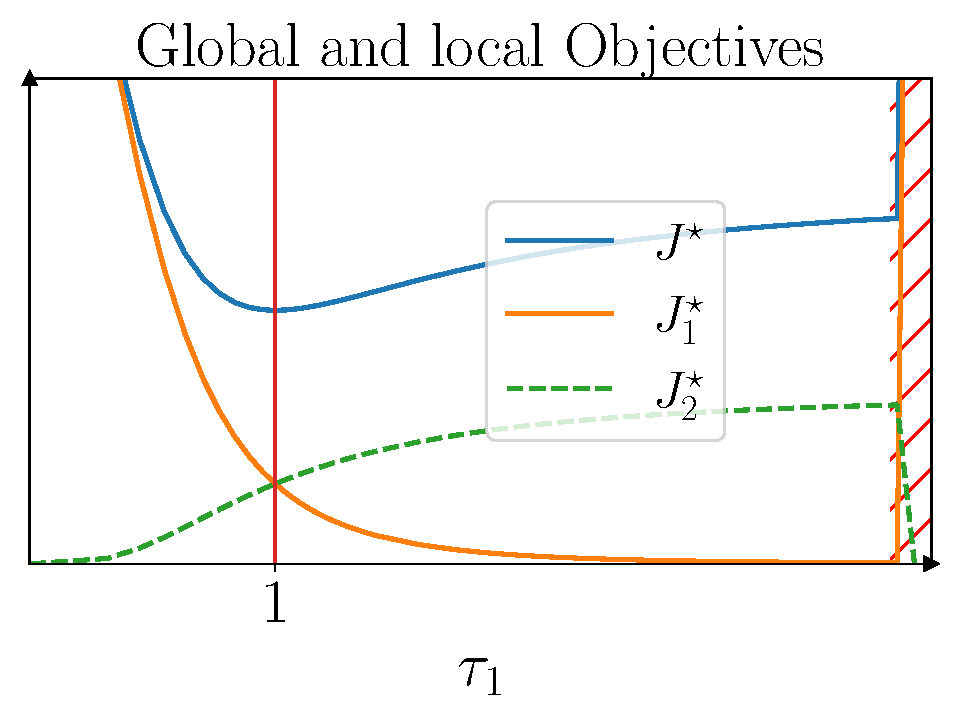
\includegraphics[width=23cm]{../img/changeOfJ.pdf}
                % \caption{}
              \end{figure}
            \end{minipage}
          };
          \draw[line width=.5cm,red,latex-] (10.5,-10) -- (10,-5.5) node[above] {Unstable};
          \node[draw,circle,minimum width=2cm,line width=.2cm,blue] (circle) at (-4.8,-11.5) {};
          \draw[line width=.2cm,blue,latex-] (circle) -- (-8,-19.5) node[below] {Optimal objective};
        \end{tikzpicture}
         \\[.8ex]
         {\Large \color{ietr_brightblue}\textbf{Can we mitigate the effects?}}
         \\[1ex]
         {YES! If we estimate $T_{i}[k]$ and invert it}
         \\[1ex]
         {But how??}
      \end{minipage}
    \end{center}
  \end{block}
\end{textblock}

\begin{textblock}{5.1}(\seccol,\secrow)
  \begin{block}{3. Estimating cheating matrix $T_{i}[k]$}
    \begin{center}
      \centering
      \begin{minipage}[c]{.95\textwidth}
        Local problems~\eqref{eq:local_problem} are {\bf QP}
        \\{\bf Explicit Solution} with {\bf PWA form w.r.t $\vec{\theta}_{i}$}:
        \begin{equation}
          \centering
          \begin{aligned}\label{eq:lambdafuntheta}
            \lambdaik=
            -P_{i}^{n}\thetaik-\vec{s}_{i}^{n}[k]\text{, if}\ G_{i}^{n}[k]\thetaik \preceq \vec{b}_{i}^{n}[k]
          \end{aligned}
        \end{equation}
        with $n\in\{1\until N\}$. $G_{i}^{n}[k]$ and $\vec{b}_{i}^{n}[k]$ define regions.
        \begin{remark}\label{rmk:p_constant}
          {\color{ietr_brightblue} Sensibilities $P^{n}_{i}$  are \underline{\textbf{time invariant}}.}
        \end{remark}
        \vspace{1.cm}
        \begin{assumption}
          In Region 1 \textbf{local constraints are active}:
          \begin{equation}
            \vec{\lambda}_{i}[k]=-P_{i}^{1}\thetaik-\vec{s}_{i}^{1}[k]\text{, if}\ G_{i}^{1}[k]\thetaik \preceq \vec{b}_{i}^{1}[k]
          \end{equation}
          % \mbox{with ${P_{i}^{1}={(\bar{\Gamma}_{i}H_{i}^{-1}\bar{\Gamma}_{i}\T)}^{-1}}$ and ${\vec{s}_{i}^{1}[k]=P_{i}^{1}\bar{\Gamma}_{i}H_{i}^{-1}\fik}$.}
        \end{assumption}
        \begin{assumption}
          ${\vec{\theta}_{i}=\0}$ belongs to Region $1$
        \end{assumption}
        \vskip 1cm
        Attacker {\bf modifies sensibility} ${\tilde{P}_{i}[k]=T_{i}[k]\bar{P}_{i}}$
        \vskip 1cm
        If we can know {\bf nominal} $\bar{P}_{i}^{1}$, estimating ${\tilde{P}_{i}[k]}$, we can find ${T_{i}[k]}^{-1}$:
        \begin{equation}
          \widehat{{T_{i}[k]}^{-1}}=\bar{P}_{i}^{1}{\widehat{\tilde{P}_{i}^{1}[k]}}^{-1}
        \end{equation}
        \vskip 1cm
        {\color{ietr_brightblue} {\large \textbf{But how do we estimate $\tilde{P}_{i}^{1}[k]$?}}}
        \vskip 1cm
        Enter Expectation Maximization
        \begin{itemize}
          \item Classify data in regions (latent variables)
          \item Estimates parameters using weighted LS
        \end{itemize}
        \vskip 1.2cm
        EM needs minimally excited inputs $\vec{\theta}_{i}$ and $\tilde{\vec{\lambda}}_{i}$.
      \end{minipage}
      \begin{itemize}
        \item \raisebox{-.5ex}{\begin{tikzpicture} \node[anchor=north,line width=1.5pt, inner sep=0pt, outer sep=0pt] (estimation) {During negotiation}; \draw[-,red] (estimation.east) -- (estimation.west);\end{tikzpicture}} (time dependence)
        \item Solution: estimate in a separate phase
              \begin{itemize}
                \item Generate independent points near $\vec{\theta}_{i}=\0$
                      \begin{itemize}
                        \item[] Artificial Scarcity Sampling
                      \end{itemize}
              \end{itemize}
      \end{itemize}
    \end{center}
  \end{block}
\end{textblock}

    \begin{textblock}{5.1}(10.5,\secrow)
      \begin{block}{4. Expectation Maximization }
      \begin{center}
\begin{minipage}[c]{0.95\linewidth}
          \begin{itemize}
            \item Regions are indexed by ${z\in\set{Z}=\{1\until Z\}}$
            \item Gaussian mixture (mean~\eqref{eq:lambdafuntheta} and ${\Sigma\to0}$)
            \item Parameters ${\set{P}=\setbuild{\set{P}^{z}}{z\in\set{Z}}}$, with ${\set{P}^{z}=(\tilde{P}^{z},\tilde{\vec{s}}^{z},\pi^{z})}$.
            \item Observations ${o\in\set{O}=\{1\until O\}}$ of $(\vec{\theta}_{i},\vec{\lambda}_{i})$
          \end{itemize}
          \vspace{.5cm}
          \SetKwBlock{Estep}{ E step:}{}
          \SetKwBlock{Mstep}{ M step:}{}
          \begin{algorithm2e}[h]
            \DontPrintSemicolon%
            Initialize parameters $\set{P}_{\mathrm{new}}$\;
            \Repeat{$\set{P}_{\mathrm{cur}}$ converges to a local maximum}{
              $\set{P}_{\mathrm{cur}}\gets\set{P}_{\mathrm{new}}$\;
              \Estep{
                Evaluate $\zeta_{zo}(\set{P})=\probability{\random{z}_{o}=z|\randomvec{\lambda}_{o},\randomvec{\theta}_{o};\set{P}}$\;
              }
              \Mstep{
                Reestimate parameters using:
                \begin{equation*}
                  \set{P}_{\mathrm{new}}=\arg\underset{\set{P}}{\max\!.}\
                  \expectation[{\zeta_{zo}(\set{P}_{\mathrm{cur}})}]{\ln\probability{\random{\Theta},\random{\Lambda},\random{Z};\set{P}}}
                \end{equation*}
              }
            }
            \caption{Expectation Maximization}\label{alg:em}
          \end{algorithm2e}
        \end{minipage}      \end{center}
    \end{block}
  \end{textblock}

  % \begin{textblock}{5.1}(0.,1.075)
  %   \begin{block}{5. Mitigation}
  %     Invert $T_{i}$ (Remark~\ref{rmk:p_constant} and~\eqref{eq:cheating})\\~\\
  %     \begin{center}
  %       \begin{minipage}[c]{.95\textwidth}
  %         If $\mathfrak{D}_{i}=0$, no attack:
  %         \begin{itemize}
  %           \item we can use the $\vec{\lambda}_{i}$ received
  %         \end{itemize}
  %         If $\mathfrak{D}_{i}=1$, $\vec{\lambda}_{i}$ received is \textbf{corrupted} $\to$ \textbf{\color{red} attack}
  %         \begin{itemize}
  %           \item Estimate $T_{i}^{-1}$:
  %                 \begin{equation}
  %                   \widehat{{T_{i}(k)}^{-1}}=\bar{P}_{i}^{1}{\widehat{\tilde{P}_{i}^{1}}[k]}^{-1}
  %                 \end{equation}
  %           \item Reconstruct $\vec{\lambda}_{i}$:
  %                 \begin{equation}
  %                   \label{eq:lambda_reconstruction}
  %                   {\vec{\lambda}_{i}}_{\mathrm{rec}}=\widehat{{T_{i}[k]}^{-1}} \tilde{\vec{\lambda}_{i}}
  %                 \end{equation}
  %         \end{itemize}
  %       \end{minipage}
  %     \end{center}
  %   \end{block}
  % \end{textblock}

  \begin{textblock}{5.1}(\thirdcol,1.17)
    \begin{block}{5. Secure dMPC}
      \begin{center}
        \begin{minipage}[c]{.965\textwidth}
          Modified negotiation (some additional steps):

          \begin{enumerate}
            \item {\bf Detection Phase}
                  \begin{enumerate}
                    \item Estimate sensibility $\widehat{\tilde{P}_{i}^{1}}[k]$
                          \begin{itemize}
                            \item Artificial Scarcity Sampling + EM
                          \end{itemize}
            \item Detect attack if $\|\widehat{\tilde{P}_{i}^{1}}[k]-\bar{P}_{i}^{1}\|_{F}\geq\epsilon_{P}$
                  \end{enumerate}
                  \item {\bf Negotiation Phase}
                  \begin{enumerate}
                    \item If detected reconstruct $\vec{\lambda}_{i}$
                  \begin{equation}
            \label{eq:lambda_reconstruction}
            {\vec{\lambda}_{i}}_{\mathrm{rec}}=\widehat{{T_{i}[k]}^{-1}} \tilde{\vec{\lambda}_{i}}
          \end{equation}
            \item Use adequate $\lambda_{i}$ to update $\theta_{i}$ \eqref{eq:negotiation}
                  \end{enumerate}
          \end{enumerate}
      %     \vspace{1cm}
      % \SetKwBlock{negotPhase}{ Negotiation Phase:}{}
      % \SetKwBlock{detectPhase}{ Detection Phase:}{}
      %   \begin{algorithm2e}[h]
      %     \DontPrintSemicolon
      %     \detectPhase{
      %       Coordinator sends sequence of $\vec{\theta}_{i}^{o}$, $o\in\set{O}$ \;
      %       Agents solve~\eqref{eq:local_problem}, and send $\tilde{\vec{\lambda}}^{o}_{i}$, $o\in\set{O}$\;
      %       Coordinator estimates $\widehat{\tilde{P}_{i}^{1}}[k]$ with \EM{} Alg.~\ref{alg:em}\;
      %       Coordinator computes $\mathfrak{D}_{i}$ using~\eqref{eq:2}\;
      %     }
      %     \negotPhase{
      %       Apply P.D. with adequate versions of $\vec{\lambda}_{i}\p$:\;
      %       \quad$\tilde{\vec{\lambda}}_{i}\p$, if $\mathfrak{D}_{i}=0$ and ${\vec{\lambda}_{i}}_{\mathrm{rec}}$, if ${\mathfrak{D}_{i}=1}$~\eqref{eq:lambda_reconstruction}\;
      %     }
      %     Apply first control in all agents
      %     \caption{Modified negotiation.}\label{alg:safeDMPC}
      %   \end{algorithm2e}
      %   \vspace{.5cm}
      \end{minipage}
      \end{center}
    \end{block}
  \end{textblock}

  % \begin{textblock}{5.1}(\thirdcol,-.075)
  %   \begin{block}{7. Expectation Maximization}
  %     \begin{center}
  %       \begin{minipage}[c]{0.95\linewidth}
  %         \begin{itemize}
  %           \item Each zone has a different ${z\in\set{Z}=\{1\until Z\}}$
  %           \item Gaussian mixture (mean~\eqref{eq:lambdafuntheta} and ${\Sigma\to0}$)
  %           \item Parameters ${\set{P}=\setbuild{\set{P}^{z}}{z\in\set{Z}}}$, with ${\set{P}^{z}=(\tilde{P}^{z},\tilde{\vec{s}}^{z},\pi^{z})}$.
  %           \item Generate $O$ observations close to $\0$
  %         \end{itemize}
  %         \vspace{1.cm}
  %         \SetKwBlock{Estep}{ E step:}{}
  %         \SetKwBlock{Mstep}{ M step:}{}
  %         \begin{algorithm2e}[h]
  %           \DontPrintSemicolon%
  %           Initialize parameters $\set{P}_{\mathrm{new}}$\;
  %           \Repeat{$\set{P}_{\mathrm{cur}}$ converges}{
  %             $\set{P}_{\mathrm{cur}}\gets\set{P}_{\mathrm{new}}$\;
  %             \Estep{
  %               Evaluate $\zeta_{zo}(\set{P})=\probability{\random{z}_{o}=z|\randomvec{\lambda}_{o},\randomvec{\theta}_{o};\set{P}}$\;
  %             }
  %             \Mstep{
  %               Reestimate parameters using:
  %               \begin{equation*}
  %                 \set{P}_{\mathrm{new}}=\arg\underset{\set{P}}{\max\!.}\
  %                 \expectation[{\zeta_{zo}(\set{P}_{\mathrm{cur}})}]{\ln\probability{\random{\Theta},\random{\Lambda},\random{Z};\set{P}}}
  %               \end{equation*}
  %             }
  %           }
  %           \caption{Expectation Maximization}\label{alg:em}
  %         \end{algorithm2e}
  %       \end{minipage}
  %     \end{center}
  %   \end{block}
  % \end{textblock}


  \begin{textblock}{15.6}(.0,3.9)
    \begin{block}{6. Example | 4 distinct rooms | 3 scenarios (Nominal, Selfish, Selfish + Correction) }
      \small
      \begin{minipage}[c]{27cm}
        \centering
        \begin{figure}[h]
          \tiny
          \begin{tikzpicture}[european]
            \node[color=mpc_agent] (house1) at (0,0) {\scalebox{3}{\faHome}};
            \node[minimum height=1cm,below=of house1] (medium) {};
            \node[color=mpc_agent,right=of medium] (house2)  {\scalebox{3}{\faHome}};
            \node[color=mpc_agent,below=of medium] (house3)  {\scalebox{2.5}{\faHome}};
            \node[color=mpc_agent,left=of medium] (house4)  {\scalebox{4}{\faHome}};
            \node[] at (house4.south) {\color{red}\scalebox{2.5}{\faUserSecret}};

            \draw[-,line width=3pt] (house1) -- (medium.center);
            \draw[-,line width=3pt] (house2) -- (medium.center);
            \draw[-,line width=3pt] (house3) -- (medium.center);
            \draw[-,line width=3pt] (house4) -- (medium.center);
            \draw[color=black,fill=mpc_coordinator,] (medium) circle [radius=.5cm];


            \begin{scope}[xshift=8cm,yshift=-2cm]
              \draw (3.,0) circle (5.5cm) coordinate (mycircle) ;
              \draw (0,0) node[tlground]{} to[isource, l=$P^{\text{heat}}$] ++(0,2)
              to[short, -*] ++(1.5,0) coordinate (a);

              \draw (a) node[above]{$T^{\text{in}}$}  to[C=$C^{\text{air}}$] ++(0,-2) node[tlground]{};
              \draw (0,-3) node[tlground]{} to[isource, l=$I^{\text{sol}}$] ++(0,2)
              to[short, -*] ++(1.5,0) coordinate (b);
              \draw (b) to[C=$C^{\text{walls}}$] ++(0,-2) node[tlground]{};

              \draw (a) -- ++(2,0) coordinate (c) -- ++(0,-.5) to[R=$R^{\text{iw/ia}}$] ++(0,-2) -- ++(0,-.5) coordinate (d);

              \draw (b) node[above]{$T^{\text{walls}}$} to[short,-*] (d);

              \draw (c) --  ++(2.5,0) -- ++(0,-.5) to[R=$R^{\text{oa/ia}}$] ++(0,-2) -- ++(0,-.5) coordinate (e);

              \draw (d) to[R=$R^{\text{ow/oa}}$] (e) to[battery,l=$T^{\text{out}}$] ++(0,-2) node[tlground]{};
            \end{scope}
            \draw[-,line width=1pt] (house2.east |- {$(house2.east)+(0,.35cm)$}) -- ( mycircle -| {$(mycircle)+(-5.5,0)$});

          \end{tikzpicture}
          \caption{3R-2C Thermic Model.}
        \end{figure}
        % \begin{table}[h]
        %   \caption{Objective functions $J_{i}$ (\% error)}\label{tab:costsGlobalLocal}
        %   \begin{tabular}[t]{cccc}
        %     \toprule
        %     Agent  & Nominal & Selfish & + Correction\\
        %     \midrule
        %     I & $ 35008.7 $ ($ 0.0 $)& $ 21969.6 $ ($ -40.0 $)& $ 35008.7 $ ($ -0.0 $)\\
II & $ 29495.3 $ ($ 0.0 $)& $ 38867.4 $ ($ 30.0 $)& $ 29495.4 $ ($ 0.0 $)\\
III & $ 24808.7 $ ($ 0.0 $)& $ 33266.4 $ ($ 30.0 $)& $ 24808.7 $ ($ 0.0 $)\\
IV & $ 23457.8 $ ($ 0.0 $)& $ 31511.0 $ ($ 30.0 $)& $ 23457.8 $ ($ 0.0 $)\\
Global & $ 112770.6 $ ($ 0.0 $)& $ 125614.4 $ ($ 10.0 $)& $ 112770.6 $ ($ -0.0 $)
\\
        %     % % Global & $ 112770.6 $ ($ 0.0 $)& $ 125614.4 $ ($ 10.0 $)& $ 112770.6 $ ($ -0.0 $)
\\
        %     \bottomrule
        %   \end{tabular}
        % \end{table}
        \begin{figure}[h]
          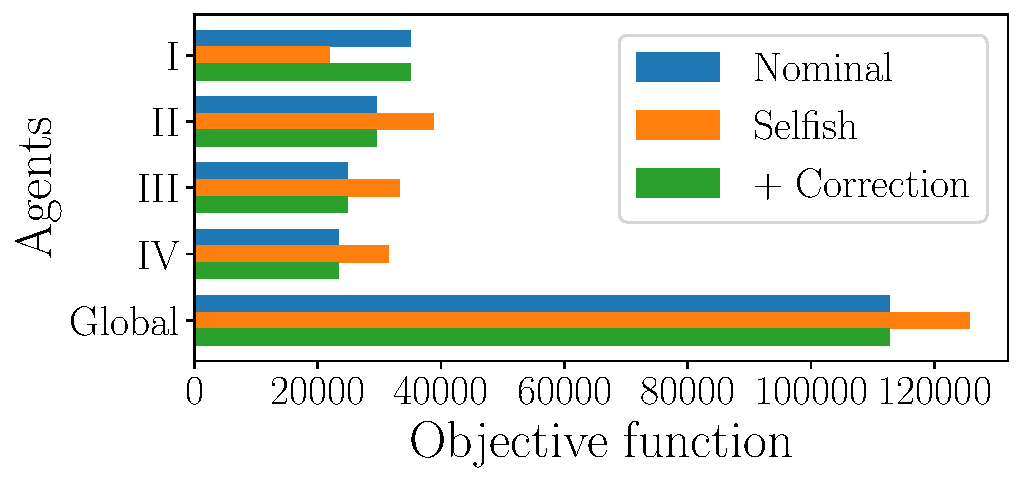
\includegraphics[width=\textwidth]{../img/barplot_results_poster.pdf}
        \end{figure}
      \end{minipage}
      \hfill
      \begin{minipage}[c]{26cm}
        \begin{figure}[h]
          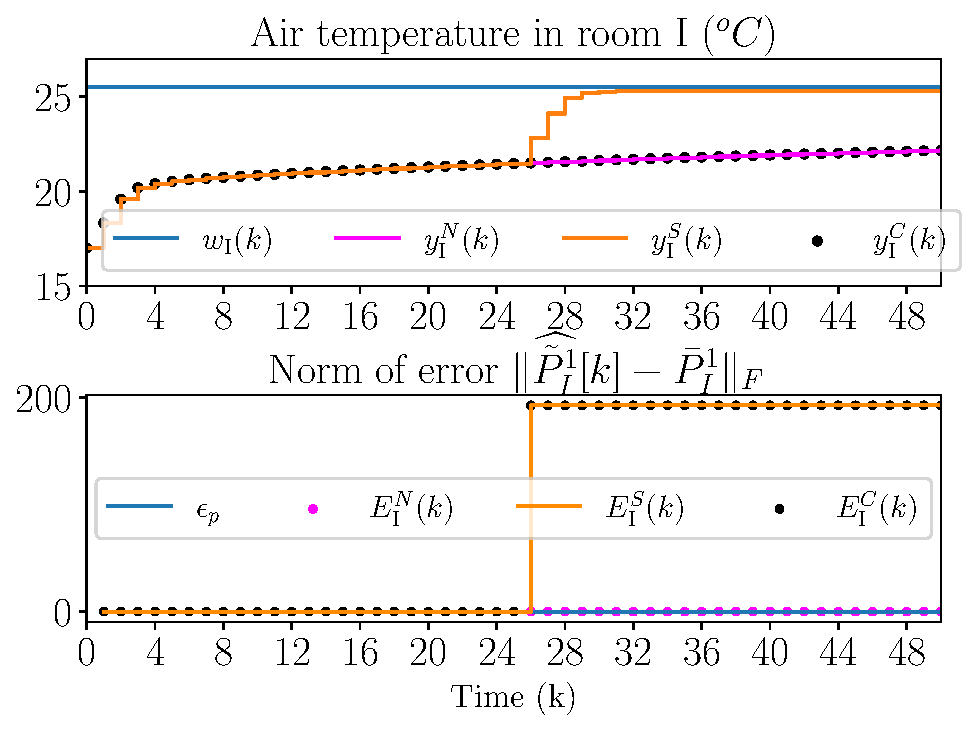
\includegraphics[width=\textwidth]{../img/airtemp_roomI/__ErrorWX_command_normErrH_poster.pdf}
          \caption{\centering Air temperature in room I and the decision variable $E_{I}[k]$ for three scenarios: nominal (N), selfish behavior (S),
            and selfish behavior with correction (C).}\label{fig:response3Scenarios}
        \end{figure}
      \end{minipage}
      \hfill
      \begin{minipage}[c]{26cm}
        \begin{figure}[h]
          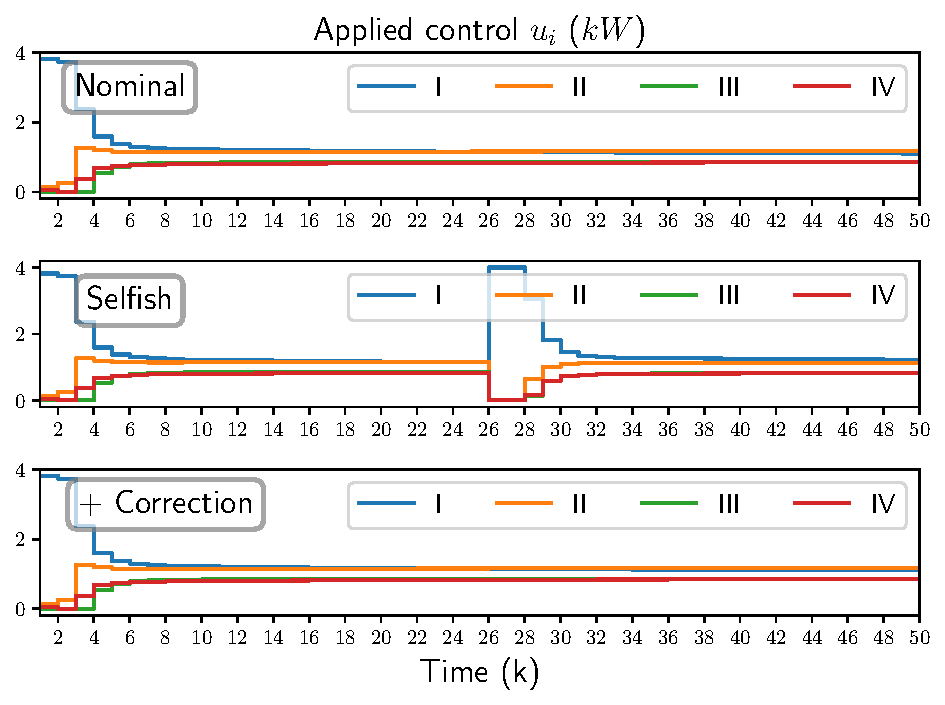
\includegraphics[width=\textwidth]{../img/airtemp_roomI/control_poster.pdf}
          \caption{\centering Control applied in all rooms for the 3 scenarios.}\label{fig:control_3Scenarios}
        \end{figure}
      \end{minipage}
      \hfill
    \end{block}
  \end{textblock}

  \begin{tikzpicture}[overlay]
    \node[] (conf_logo) at (.15\paperwidth,-.515\paperheight) {
\includegraphics[width=.25\textwidth]{../img/logo_NecSys.png}};
    \node[right=of conf_logo,align=right]  {\bf Zurich, Switzerland \\5-7 July 2022};
  \end{tikzpicture}

\end{frame}

\end{document}
